\documentclass[12pt, letterpaper]{report}
\usepackage[style=authoryear, maxnames=2, maxbibnames=99, citestyle=apa]{biblatex}
\addbibresource{merged_biblio2.bib}
\addbibresource{internet_stuff.bib}
\usepackage{caption}
\usepackage{geometry}
\usepackage{graphicx}
\usepackage{setspace}
\usepackage{ulem}
\usepackage{url}
\usepackage{lineno}
\usepackage{tabularx}
\usepackage{gensymb}
\usepackage{longtable}
\usepackage{titlesec}
\usepackage{subcaption}
\usepackage{pdflscape}
\usepackage{booktabs}
\usepackage{array}
\usepackage{fancyhdr}
\usepackage{chemformula}
\usepackage[hidelinks]{hyperref}
\pagestyle{fancy}
\fancyhf{}
\renewcommand{\headrulewidth}{0pt}
\fancyfoot[R]{\thepage}
\fancypagestyle{plain}{%
\fancyhf{}%
    \renewcommand{\headrulewidth}{0pt}%
    \fancyfoot[R]{\thepage}%
}

% Modify the fancy page style for chapters
\fancypagestyle{fancy}{%
    \fancyhf{}%
    \fancyfoot[R]{\thepage}%
}

\newcommand{\mycomment}[1]{}

\titleformat{\chapter}[block]{\Large\bfseries}{Chapter \thechapter.}{20pt}{\raggedright\Large}
\titlespacing{\chapter}{0pt}{5pt}{5pt}
% Adjust section spacing to prevent orphans
\titleformat{\section}{\large\bfseries}{\thesection}{1em}{\large}
\titlespacing*{\section}{0pt}{\baselineskip}{0.5\baselineskip}

% Adjust subsection spacing to prevent orphans
\titleformat{\subsection}{\normalsize\bfseries}{\thesubsection}{1em}{\normalsize}
\titlespacing*{\subsection}{0pt}{\baselineskip}{0.5\baselineskip}

\graphicspath{./images/}
\geometry{
        letterpaper,
        top = 2.54cm,
        bottom = 2.54cm,
        left = 2.54cm,
        right = 2.54cm,
        }
\title{MSc Thesis}
\author{Isaac Peetoom Heida}
\date{December 2022}
\doublespace

\begin{document}
\pagenumbering{roman}
\setcounter{page}{2}
\begin{titlepage}
    \begin{center}
        \vspace*{1cm}

        \textbf{Ecological and genetic drivers of silicon accumulation in cereal crops}

        \vspace{1cm}

        by 

        \vspace{1cm}

        \textbf{Isaac Peetoom Heida}
        
        \vfill

        \textsc{a thesis submitted in partial fulfillment of the requirements for the degree of}

        \vspace{1cm}

        \textsc{master of science}

        in

        \textsc{the faculty of graduate and postdoctoral studies}

        (Plant Science)

        \textsc{the university of british columbia}

        (Vancouver)

        August 2023

        \copyright Isaac Peetoom Heida, 2023
    \end{center}
\newpage

\end{titlepage}
\thispagestyle{plain}
\setcounter{page}{2}
{
%\setlength{\parskip}{12pt}
%\begin{adjustwidth}{0pt}{0pt}
\vspace{1cm}

\noindent The following individuals certify that they have read, and recommend to the Faculty of Graduate and Postdoctoral Studies for acceptance, the thesis entitled:

\vspace{1cm}

\noindent \uline{Ecological and Big Genetic Drivers of Silicon Accumulation in Cereal Crops\hfill}
%\hfill\rule{\textwidth}{0.4pt}

\vspace{1cm}

\noindent submitted by
%\rule{\textwidth}{0.4pt}
\noindent \uline{Isaac Peetoom Heida\hfill}
\noindent in partial fulfilment of the requirements for 

\vspace{1cm}
\noindent the degree of \uline{Master of Science\hfill}

\vspace{1cm}
\noindent in \uline{Plant Science\hfill}

\vspace{1cm}

\noindent \textbf{Examining Committee}:

%\vspace{1cm}

\noindent \uline{Juli Carrillo, Professor, Plant Science, UBC\hfill}

%\rule{\textwidth}{0.4pt}

\noindent \textit{Supervisor}

\vspace{1cm}

\noindent \uline{Gurcharn Singh Brar, Professor, Plant Science, UBC\hfill}

%\rule{\textwidth}{0.4pt}

\noindent \textit{Supervisory Committee Member}

\vspace{1cm}

\noindent \uline{Jean-Thomas Cornelis, Professor, Soil Science, UBC\hfill}

%\rule{\textwidth}{0.4pt}

\noindent \textit{Supervisory Committee Member}
%\end{adjustwidth}
}

% Rest of your document





\chapter*{Abstract}
\addcontentsline{toc}{chapter}{Abstract}

Over the past 30 years, the potential of silicon to improve crop plant performance has gained increasing recognition in the field of plant science. Silicon may be a key tool to guard crop production against uncertain future growing conditions by improving crop tolerance to abiotic and biotic stressors. In this thesis, I take recent advances in our understanding of silicon ecology and extend them into cereal crops, testing for the presence of rapid ($<24$ hour) silicification in common Canadian crops after defence induction events, including herbivory, and used a genome-wide association study to identify potential genetic markers associated with high silicon content. We found that overall, simulated herbivory, but not cricket herbivory, increased silicon leaf content. However, at the species level, we found no significant increases in silicon content in response to herbivory treatments. This may be due to a silicon-poor soil environment or could reflect the effect of herbivore identity on specific defensive outcomes. In our genetic analysis, we found no genetic markers with significant associations to silicon content but did find a marker that had a significant correlation with manganese content. Our limited results may reflect the polygenic nature of silicon content in plants, or strong environmental effects. Future studies could build upon our results by developing a mapping population using genotypes we identified as representing the extremes of silicon content. Applications of silicon research into crop production techniques are still limited by crucial gaps in our understanding of how ecology and genetics control silicon uptake, but this work provides yet another steppingstone towards the broader adoption of silicon into agricultural systems.

\chapter*{Lay Summary}
\addcontentsline{toc}{chapter}{Lay Summary}

Silicon provides tremendous benefits to plant health but is not yet widely utilized in agriculture despite it being highly abundant and naturally occurring in most soils. Silicon acts as a defensive compound against insects, and helps plants deal with stressful growing conditions, but is not currently widely applied in agriculture. Using cereal crops and a wild ancestor of wheat, I attempted to identify ecological and genetic factors that drive silicon content.  We failed to find genetic regions that exerted control over silicon content but observed large variations in silicon content between the growing sites. We did not observe short-term silicon uptake in our tested cereal crops, complicating our understanding of when short-term silicon accumulation is achieved by plant species. Continuing to build upon this research will help move silicon crop technologies closer to feasibility and could provide an environmentally friendly strategy to reduce pesticide use while maintaining yields.

\chapter*{Preface}
\addcontentsline{toc}{chapter}{Preface}

The research presented in this thesis is original and unpublished. Isaac Peetoom Heida and Dr. Juli Carrillo, with assistance from Dr. Jean-Thomas Cornelis and Dr. Gurcharn Singh Brar, conceptualized and developed the experiment presented in Chapter Two. Isaac Peetoom Heida, Dr. Juli Carrillo and Dr. Gurcharn Singh Brar, with input from Dr. Jean-Thomas Cornelis, conceptualized and developed the experiment presented in Chapter Three.
Isaac Peetoom Heida developed the question and methodology for Chapter Two. Dr. Aaron Beattie, Dr. Mazen Aljarrah, and Dr. Gurcharn Brar provided seeds for the experiment. Isaac Peetoom Heida designed and set up the experiment, processed and analysed the samples, and performed the statistical analysis. Dr. Shaun Barker and the Mineral Deposit Research Unit of the University of British Columbia provided facilities and expertise for the XRF analysis of the tissue samples. Dr. Simone Castellarin and Dr. Joana Pico Carbajo provided facilities and guidance in developing the protocol for phenolic analysis. Chelsea Gowton provided indispensable assistance with phenolic sample processing. 
For Chapter Three, Isaac Peetoom Heida led planting, plot setup, and maintenance, with assistance from Grace Wang, Vincent Fetterley, Sara Salad, Katherine Buchanan, Martina Clausen, Paul Fisher, and Matt Tsuruda. Isaac Peetoom Heida led the sample harvest, processing and analysis. Kelly Wang, Grace Wang, and Chelsea Gowton assisted with the sample harvesting. Dr. Daria Reshetniak, Paul Fisher, Lucas Friesen, Katie Pryer, Dr. Kinga Treder, Chelsea Gowton, Dennis Chiu, Carly MacGregor, and Grace Wang all provided invaluable assistance with sample preparation. 
I use the first-person plural for chapters two and three as they are intended for submission to a peer-reviewed journal. 

\newpage
\tableofcontents
\newpage
\listoftables
\newpage
\listoffigures

\chapter*{Acknowledgements}
\addcontentsline{toc}{chapter}{Acknowledgements}

This work would not have happened without the continuous support of my committee, the members of the PIEE lab, my friends and family, and the generosity of a host of funding agencies. Dr. Juli Carrillo has guided me to become a more well-rounded scientist and person and has always believed in my abilities. I thank Dr. Jean-Thomas Cornelis for providing the silicon spark to kick this entire project off. Dr. Gurcharn Singh Brar lent his time and lab to me to support the work and stoked my passion for grasses from a new angle. The members of the PIEE lab were more than generous with their time, and their continued interest in my project and general conviviality provided the encouragement I needed to keep going with my research. In some ways this work is the culmination of a lifetime of support from my family, as they encouraged my curiosity about the natural world and sought out opportunities for me when I was too young (or too dumb) to seek them out for myself. Lastly, NSERC, CPBI, and the UBC provided generous scholarships and fellowships in support of my research and personal development.

\chapter*{}
\addcontentsline{toc}{chapter}{Dedication}

\noindent{\Large\textit{To my Auntie Margaret, for showing me where the wetland was all those years ago.}}

\chapter{Introduction}
\pagenumbering{arabic}

\section{A case for silicon in agriculture}

As global agricultural production strains under degrading soil fertility and increasing losses due to climate change, new technologies are being developed for sustainable improvement in crop production. New crop technologies will meet increasing public and regulatory demand for environmental sustainability, encouraging scientists to revisit overlooked or relatively unknown techniques that may unlock productivity gains. Over the past 30 years, plant-silicon relations has emerged as a promising field that may safeguard crop performance and security within a changing biosphere. With benefits to multiple dimensions of crop performance, silicon may be a key tool to guard crop production against uncertain future growing conditions. 

\section{Silicon in Soils}

Silicon abounds in the earth’s crust, with various silicates, such as silicon dioxide (\ch{SiO2}), comprising about 60\% of the crust by mass (\cite{holland_41_2014}). Nearly all terrestrial plants grow in soils containing silicon, and thus absorb at least nominal amounts through passive transport as the plant absorbs water (though many plants have active transport) (\cite{debona_silicons_2017}). Silicates occur in a variety of forms and vary in their plant availability. Crystalline forms, such as quartz, are highly resistant to weathering, and are poor sources of plant-available silicon, while amorphous forms of \ch{SiO2} are more available (\cite{fraysse_surface_2009}). 
Plants interact with silicon on a variety of levels, mobilizing it from soil aggregates, transporting it into and throughout their bodies, and finally precipitating it out of the xylem into solid masses in the leaves and stems. Within the soil environment, silicon commonly exists in both crystalline (geologic) and amorphous (biogenic) forms (Haynes 2014). Amorphous silicates can derive from previous plant material that has decayed in the soil, but also from marine and aquatic organisms such as diatoms. Young soils typically have high fractions of silicon-bearing materials, including clay minerals, though plant-available silicon peaks in middle-age soils (~120,000 years old) (\cite{de_tombeur_silicon_2020}). The continual leaching of silicon from terrestrial sediments over geologic timescales means as ecosystems age, plants become more and more central in the local silicon cycle, with much of the silicon in living plant tissue being recycled from previous plant material decaying in the soil (\cite{de_tombeur_plants_2020}).  

\section{Plant uptake of silicon}

One of the most important advances in plant-silicon research was understanding the mechanisms through which plants acquire and transport silicon to specific locations within the plant (\cite{coskun_controversies_2019}). Silicon’s most common form in soil solution is silicic acid (\ch{H_4SiO_4}), which has a maximum solubility of around 2 mM (\cite{haynes_contemporary_2014}). In highly weathered soils with low nutrient availability, plants take a more active role in liberating nutrients, and other elements, including silicon, for uptake. Organic acids and chelating agents, exuded from plant roots, pry tightly bound nutrients and beneficial elements such as phosphorus and silicon from soil aggregates, increasing their availability for uptake into the root system (\cite{de_tombeur_silicon_2021-1}). Once dissolved in soil solution, silicon can be taken up by active or passive transport by the root system. While there is some evidence that small amounts of silicic acid can be transported during water uptake, this method of transport is insufficient to explain the larger amounts of silicon found in some plant families. 

Research in rice has identified four gene products that actively transport silicon into and through the plant body. Two of these (LSi1, LSi2) transport silicic acid from the soil into the roots, while the other two (LSi3, LSi6) act to unload silicic acid from the xylem into leaves and inflorescences (\cite{yamaji_orchestration_2015}). Orthologs of these proteins have been identified in other cereal crops, and additional analogous silicon transporter proteins have been discovered in the Cucurbitaceae (\cite{reynolds_silicon_2016}). Though not identified, there is a hypothesized fifth protein responsible for loading silicic acid into the xylem (\cite{farooq_silicon_2015}). Throughout the plant kingdom, clades vary significantly in their silicon content and expression of silicon transporter proteins (\cite{ma_chapter_2001}). The expression of these genes, or lack-there-of, can not only influence the total amount of silicon accumulated by the plant, but also its relative distribution, as knockout of LSi6 increases leaf silicon content while decreasing the silicon content of seed husks in rice (\cite{yamaji_transporter_2008,yamaji_orchestration_2015}). Breeding for silicon content, improved exudate-based silicon mobilisation and silicon use-efficiency in crop plants may be crucial to improving crop performance under a changing climate (\cite{de_tombeur_silicon_2021,christian_breeding_2022}). However, we still have a relatively poor understanding surrounding how genetics influence the silicon phenotype of a plant. Further investigations into how genotypic variation is reflected in the silicon content of plants can aid in the discovery of new genes involved in silicon accumulation and may provide targets for silicon breeding programs. 

\section{Silicon in the plant body}

Plants deposit silicon in specialized silica cells, forming phytoliths (\cite{waterman_short-term_2021-1}). Silicon deposits show taxa-specific morphologies, suggesting evolutionary pressure selecting for these structures to yield certain functions to the plant (\cite{piperno_phytoliths_2006}). In stems, these phytoliths are often long and narrow, oriented parallel with the shoot, and seem to increase structural rigidity (\cite{stromberg_functions_2016}). The use of silicon as a structural component represents a highly energetically efficient strategy, as silicon is ~10x cheaper on an energy unit basis to produce than lignin (\cite{stromberg_functions_2016}). Stem silicification has been investigated as it relates to lodging resistance in cereal crops, and silicon supplementation has been found to reduce the prevalence of lodging in rice and wheat (\cite{dorairaj_influence_2017,muszynska_mechanistic_2021}). In leaves, phytoliths are typically stouter, though they still increase the mechanical toughness of the leaf (\cite{simpson_still_2017}). This overall toughness, and abundance of phytoliths in leaves is thought to have evolved to limit herbivore damage, rather than improve the growth characteristics as in stem phytoliths (\cite{stromberg_functions_2016}).

Leaf silicon concentrations are negatively correlated with relative growth rate and survival in several invertebrate herbivores (\cite{massey_silica_2006,juma_influence_2015,mir_silicon_2019}). Phytoliths act by wearing down the mandibles of insect herbivores, thus reducing feeding efficiency (\cite{mir_silicon_2019,waterman_short-term_2021-1}), as well as reducing the digestive efficiency of the herbivore gut (\cite{hunt_novel_2008}). Interestingly, even in the absence of silicon, plants develop silica cells, and rapidly fill them when silicon becomes available (\cite{waterman_short-term_2021-1}). As phytoliths develop in the leaves, polymerisation of monosilicic acid is aided by interactions with proteins in the cell wall, which act as sites of nucleation (\cite{nawaz_phytolith_2019}). Silicon deposition in the leaves can happen on relatively short time scales, outpacing the accumulation of other defensive compounds such as phenolics (\cite{waterman_short-term_2021}). Thus, silicon-based defences in crop plants may be one of the first lines of active anti-herbivore defence, providing rapid and sensitive responses to herbivory.

In addition to the anti-herbivore benefits, silicon deposition seems to provide heightened disease resistance and stress tolerance. When supplemented with silicon, plants are generally more resistant to a wide spectrum of stressors, including soil salinity, soil metal toxicity, cold and heat stress, UV stress, water deficits, and phosphorus deficiencies (\cite{cooke_consistent_2016}). Empirical evidence also shows that silicon is effective at limiting the growth of some fungal plant pathogens (\cite{fauteux_silicon_2005}). These wide-ranging positive effects may be due to silicon-based apoplastic barriers that seal and toughen the plant tissue (\cite{coskun_controversies_2019}). Under this apoplastic barrier hypothesis, silicon deposits reduce water loss and radiation/temperature damage, and limit the spread of effector compounds, dampening the effects of fungal pathogen and herbivore excretions designed to interfere with plant defensive physiology (\cite{coskun_controversies_2019}). Continuing to untangle the various mechanisms through which silicon delivers beneficial effects to plants is key to fully realizing the potential of silicon in sustainable agriculture.

\section{Looking back and looking forward}

Much of today’s plant silicon work is indebted to the pioneering work of \textcite{jones_silica_1967}, who published a comprehensive study of silica in biotic systems, and the subsequent charting of silicon content across the plant kingdom by \textcite{takahashi_possibility_1990}. Epstein’s \citedate{epstein_silicon_1999} seminal paper provided a comprehensive review of the state of knowledge in plant silicon and has spurred a generation of researchers to extend the preliminary findings of the 20th century out across crop production systems and plant ecologies around the world (\cite{cooke_is_2011,hartley_ecology_2016,coskun_controversies_2019,de_tombeur_silicon_2021,christian_breeding_2022}). Silicon has been best studied in the grass family (Poaceae) due to the comparatively high silicon content found in most members of the family (often over 1\% of dry weight), as well as the economic importance of domesticated species within the clade (\cite{reynolds_silicon_2016}). The domesticated grass species rice, maize, wheat, and barley alone account for one-third of the worlds’ total cultivated land area (\cite{faostat}). Silicon supplementation as an agricultural practice has been extensively studied in rice and sugar cane, as these crops tend to be grown in soils naturally low in silicon, and rapidly deplete the remaining silicon stocks, necessitating replenishment by application of silicon-rich amendments (\cite{haynes_contemporary_2014,meena_case_2014}). The depletion of silicon in these production systems has spurred much research activity targeting the biology of silicon, particularly in rice (\cite{deren_variable_1992-1,dai_genetic_2005,rodrigues_silicon_2004,ye_priming_2013}). In most temperate soils globally, Si is rarely truly limiting in soils, though certain forms of silicon are much more plant available than others (\cite{fraysse_surface_2009}). Thus, silicon research has been slower to develop in dryland temperate cereal crops, (but see \cite{rains_active_2006,ahmad_silicon_2016,neu_silicon_2017}). Great work can still be done to improve the manner and efficiency in which these temperate crops utilize the ample silicon available in their soils. Our ability to integrate silicon as a tool for improving crop production is currently limited by a poor understanding of the genetic controls over silicon accumulation, as well as a limited understanding about the extent to which crops utilize silicon in pest-protection. 

%\printbibliography

\chapter{Testing rapid silicon accumulation in four cereal crops under real and artificial herbivory}

Note: this chapter has been prepared with the intention of submission to a peer-reviewed journal, and thus I use the plural first-person throughout.

\section{Introduction}

To counter acute damage from herbivores, plants have developed a host of defensive strategies, ranging from changes to the body plan to the development of novel compounds to poison organisms that try to eat the plant (\cite{agrawal_plant_2006}). Due to the vastly different nature and ontogeny of various defensive strategies in plants, plant defences operate across a range of intensities and time scales, from short-term temporary activation to long-lasting changes in the morphology of the plant (\cite{agrawal_plant_2006, karban_induced_1989}). In most scenarios, plants induce defences in response to an external cue, and build in intensity over time, with defensive hormone signals peaking approximately five hours after the initial induction event (\cite{schmelz_quantitative_2003}). Despite this rapid hormonal response, actual defensive phenotypes are slower to emerge, due to the higher costs of synthesizing defensive compounds, or developing new tissues like thorns and spines (\cite{karban_induced_1989}). Many defensive responses are also context dependent, where the identity of the damaging actor (e.g. species of insect), the severity of damage, and a host of other factors interact to determine the final defensive response (\cite{waterman_simulated_2019}). The most effective defensive strategies should be those that can either prevent herbivory outright, or rapidly respond to limit damage. These same strategies are also the most promising for crop production, where pest damage represents both an economic and food security cost. Integrating better natural plant defences into crop production systems could reduce some of the environmental impact of agriculture, but hinges upon a thorough understanding of plant defensive physiology.

One of the most promising avenues for new crop defence is the harnessing of silicon (\cite{reynolds_silicon_2016}). Silicon acts on multiple temporal and physiological scales, delivering broad spectrum resistance to pests, pathogens, and abiotic stressors (\cite{cooke_consistent_2016,coskun_controversies_2019}). Soluble silicon taken up from the soil is deposited predominantly in the leaf epidermis, where it forms solid granules that increase the toughness of the tissue, reducing herbivore digestive efficiency (\cite{cooke_is_2011}). Nearly all plants accumulate silicon over their lifespans, but there is also evidence of more acute silicon accumulation in response to herbivory (\cite{takahashi_possibility_1990}).

Multiple studies have demonstrated lasting elevated silicon in response to real and simulated herbivory (\cite{massey_are_2008,hartley_ecology_2016}), with much of the silicon accumulation occurring in the days after the herbivory cue (\cite{ye_priming_2013}). Recent evidence points to silicon accumulation as being a relatively rapid response, increasing by up to 30\% within six hours after defensive cues, outpacing increases in phenolic compound-based defences (\cite{waterman_short-term_2021}). This rapid action makes herbivory-induced silicon accumulation a promising trait for future crop development. Despite the novel results, this pattern has so far been observed in just one species: \textit{Brachypodium distachyion}. Testing for this rapid herbivory-induced silicon accumulation across a variety of grain crops, and under both simulated (methyl-jasmonate) and real herbivory is a crucial first step towards integrating rapid silicification into our understanding of plant defence and crop protection.

Plant silicon research has mostly focused on members of the grass family (Poaceae) due to their exceptional silicon content within the plant kingdom, as well as the economic importance of domesticated grass species (\cite{reynolds_silicon_2016}). Much of the research on silicon-herbivore interactions used wild species, yet domesticated crops differ significantly from their wild relatives, due to effects of strong selective pressure imposed by humans (\cite{chen_crop_2015}). Most domesticated crops show much lower genetic diversity than their wild ancestors (\cite{smith_domestication_2019,hafeez_creation_2021}). Initial selection for a few individuals with favourable traits creates a genetic bottleneck, and most allelic diversity is lost. Subsequent selection by humans for agronomically relevant traits can result in concurrent losses of adaptations to natural environments, as the traits that maximize human value (e.g., yield, ease of harvest) can come at the cost of ecologically relevant traits such as defence (\cite{chen_crop_2015,whitehead_domestication_2017}). Indeed, in the context of silicon, we can detect clear signals of domestication across the Poaceae family, where wild ancestors consistently have higher baseline silicon content than their domesticated descendants (\cite{simpson_still_2017}). Novel findings and developments in the silicon-herbivore literature need to be tested with modern crop species, both to validate their utility towards agricultural production, and to gather further observations on the dynamics of silicon-based defences in a broader set of species.

In this study, we tested cultivars of four globally important cereal crop species for rapid herbivory-induced silicon accumulation under artificial and real herbivory. In a glasshouse environment, we grew bread wheat (Triticum aestivum), oats (Avena sativa), barley (Hordeum vulgare) and Triticale (x Triticosecale), and tested the following hypotheses:
\begin{enumerate}
        \item Rapid silicon accumulation is a conserved trait in the Poaceae, and the tested species' silicon content would show a significant increase in silicon content within 18 hours of the herbivory treatment applications.
        \item Due to disparate taxonomic origins, the tested species would vary in the strength of their silicon accumulation response to herbivory. 
        \item Due to the different cues involved when comparing true herbivory damage and methyl-jasmonate induced defensive induction, the tested species would show different patterns of short-term silicon accumulation in response to cricket (Acheta domesticus) herbivory and methyl-jasmonate application. 
\end{enumerate}
This study is a thematic replication of Waterman et al.’s 2021 paper, which found \textit{Bracypodium distachyon} accumulated silicon within six hours after methyl-jasmonate application and that silicon was faster to accumulate than phenolic compounds. We attempt to extend these findings to commercially important grain crops. The findings of this study will refine our understanding of the prevalence of rapid silicification in the Poaceae and will help to inform the value of potential applications of silicon-based defences into grain crops.

\section{Methods}

\subsection{Plant growth and experimental treatments}

To test the prevalence of rapid silicon accumulation in Canadian cereal crops, we selected three cultivars each of oats, bread wheat, triticale, and barley (Figure \ref{Fig:exp_design}). We selected cultivars based on minimizing shared pedigree, and no cultivars shared more than one common ancestor within the last two crossing generations. At the start of the experiment, we germinated seeds in germination trays filled with moist sand. After four days, we transplanted germinated seedlings into 10 cm pots filled with SunGro Sunshine Mix \#4 amended with 0.17 g of solid silicic acid (a rate of 2.4 g silicon / kg of soil). Though potting mix and fresh water contain some amount of plant available silicon, we added the silicic acid to reduce silicon limitation to the plants. We randomized the location of each pot within the growing space. A flood table bottom watered the pots with nutrient solution. We assigned each plant to one of three herbivory treatments: control, simulated herbivory, or cricket herbivory. We simulated herbivory by application of 1 mM methyl-jasmonate solution to the entire above-ground portion of the plant (\cite{waterman_short-term_2021}), while crickets housed in water-pik tubes provided true herbivory (Figure \ref{Fig:exp_design}). Prior to introduction to the plants, we acclimated crickets by feeding them for 72 hours on the same species used in this trial. We applied our treatments 45 days after transplanting. Immediately preceding cricket application, we placed the crickets in their experimental tubes and starved them for 24 hours, as this increased the likelihood of the insects initiating feeding rapidly upon exposure to the test plants. Prior to harvest, we recorded whether the crickets had initiated feeding on the plants by visually inspecting the leaves for missing tissue. 

\subsection{Sample harvest and preparation}

We harvested three fully expanded upper leaves from the plants 18 hours after treatment application and split the leaves in half along the midvein. We placed one half of the tissue into a coin envelope, oven dried it for 4 days at 60\degree C, transferred it to a 2 mL microcentrifuge tube with three 3.2 mm diameter steel beads, and ground it into a fine powder using a tissuelyser (60 seconds at 30 Hz) in preparation for silicon content analysis. We placed the other half of the tissue into a microcentrifuge tube, flash froze it in liquid nitrogen, and subsequently freeze dried it. After freeze drying, we ground the samples for phenolic processing under the same conditions as the other samples.


\subsection{Silicon analysis}

To measure the silicon content of the leaf tissue, we followed a modified version of the bench-top x-ray fluorescence (XRF) method (\cite{reidinger_rapid_2012}). We pressed leaf powder in a hydraulic press at 300 bar, using a 13 mm die to create a pellet. We then placed the pellet in an Olympus Vanta pXRF mounted in a benchtop stand, and used a 45 second scan time to quantify silicon. After each use, we cleaned the pellet die and XRF analyser to minimize contamination between samples.

\section{Phenolic analysis}

We analysed phenolics to double check the effectiveness of our methyl-jasmonate applications on defence induction and to examine the relationship between phenolics and silicon. To measure the response of phenolics to our treatments, we used the Fast Blue BB method (\cite{pico2020systematic}), scaled to use 0.075g of freeze-dried leaf tissue.  

\subsection{Statistical analysis}

Despite the starvation, some crickets did not initiate feeding during the exposure period ($\sim38\%$). We filtered out plants assigned to the insect induction treatment that received no damage, to ensure that they would not confound the model ($n = 33$). Prior to running our full model, we first tested for an effect of plant biomass on silicon content, as defence levels can be influenced by plant size (\cite{carmona_plant_2011}). We found a negative correlation between plant size and silicon content ($\beta = -0.067 \pm 0.017, p < 0.001$), and thus included plant size as a covariate in our final model. To test all three of our hypotheses, we used linear mixed effects models. We tested the responses of leaf silicon and phenolic content to the fixed effects of treatment and species, with a covariate of biomass. We used cultivar identity as a random effect, as we were interested in understanding how silicon and phenolics varied across treatments and species, but not across cultivars. We implemented these models using the following R model formulae:
\[Silicon ~ Species * Induction + Biomass + (1|Cultivar)\]
\[Phenolics ~ Species * Induction + Biomass + (1|Cultivar)\]
We assessed the models using lmerTest (\cite{kuznetsova_2017_lmerTest}) with a type III ANOVA. 
Though not directly related to our hypotheses, we conducted additional post-hoc tests investigating trade-offs between phenolic and silicon content (\cite{simpson_still_2017,waterman_short-term_2021}). We tested the relationship between silicon and phenolic content using a linear mixed effects model with the following R model formula:

\[Phenolics ~ Silicon + Species + Biomass + (1|Cultivar)\]

\subsection{Software used}

We compiled the final dataset using DataFrames.jl (\cite{bogumil_kaminski_2023_7632427})Kamiński et al. 2022) in Julia 1.9.0 (\cite{bezanson2017julia}). We tested the mixed effects models in R 4.2.2 (\cite{r_core_team_2022}) using lmerTest (\cite{kuznetsova_2017_lmerTest}) and performed a post-hoc Tukey test using emmeans (\cite{lenth_2023_emmeans}). We generated graphics in Julia using Plots.jl (\cite{tom_breloff_2023_7736124}).

\section{Results}

Among cultivars, average baseline (control treatment) silicon content ranged from 0.26\% to 0.91\% (Figure \ref{Fig:baseline_si}). Species differed in silicon content ($species: p = 0.012, F = 6.08, df = 3,10.3$) with the lowest average silicon content at $0.34 \pm 0.02\% (mean \pm SE)$ in oats, and  the highest average silicon content at $0.76 \pm 0.05\% (mean \pm SE)$ in wheat (Figure \ref{Fig:baseline_si}). Silicon content varied by induction treatment ($induction: p = 0.011, F = 4.62, df = 2,186$, Table \ref{Tab:si_params}) with higher silicon content in plants exposed to methyl-jasmonate, while insect and control plants had similar silicon content (Figure \ref{Fig:induction_across_spp}). Within species, we did not see induced silicon accumulation for either methyl-jasmonate application nor insect feeding (Figure \ref{Fig:induction_by_spp}), however wheat had significantly lower silicon with cricket feeding, leading to a significant interaction between species and induction ($interaction: p=0.040, F = 2.52, df = 6,186$). 

We found a significant effect of species, but not induction treatment, on phenolic content (Figure \ref{Fig:induction_by_spp}, Table \ref{Tab:phe_params}). Oats had the highest average leaf phenolic content $(31.9 \pm 3.66 mg/g) (mean \pm SE)$, while barley had the lowest average phenolic content $(12.9 \pm 1.82 mg/g) (mean \pm SE)$. We did not find a significant relationship between silicon and phenolic content ($p = 0.15$), despite an apparent negative trend in the scatter plot (Figure \ref{Fig:phe_si_scatter}).

\section{Discussion}

Recent research in inducible silicon plant defences has focused on the short-term ($<24$ hours) dynamics of herbivory-triggered silicon uptake (\cite{waterman_short-term_2021,waterman_short-term_2021-1}). The promising results of this work have been highlighted for their potential applications in agriculture, where sensitive and rapid defensive phenotypes could improve plant performance and reduce reliance on more intensive pest-control measures. In this study, we assessed rapid silicification in four cereal crops. We failed to find evidence of rapidly induced silicon uptake in response to either methyl-jasmonate application or herbivore feeding within any of the species tested. Despite our model showing significant effects of both treatment and species on the silicon content, comparing across treatments we see only a slight trend towards increased silicon content, with methyl-jasmonate treated plants displaying the highest silicon content, while control and insect-treated plants had lower silicon content. Surprisingly, in wheat the insect treatment resulted in the lowest silicon content. Silicon deposition is a permanent process; plants cannot remobilize silicon once it has been deposited. It is virtually impossible that cricket feeding on wheat led to a plant response of decreasing silicon. However, this pattern may be a signal of silicon-content based feeding preferences, which we discuss more in depth farther below.

This study differed from previous studies demonstrating rapid herbivory-induced silicon uptake in several ways. The two previous studies (\cite{waterman_short-term_2021,waterman_short-term_2021-1}) both grew plants in liquid nutrient solution, carefully standardized to maintain consistently high silicon availability. In our study, we grew plants in potting soil amended with solid silicic acid, similar to \textcite{nascimento_silicon_2019}. In natural soil environments, most plant-available silicon is derived from mineral or biogenic sources, and thus requires dissolution into the soil solution (\cite{de_tombeur_silicon_2021-1}). The maximum concentration of silicic acid in soil solution is 2mM, however observed concentrations can be much lower. Phytoliths (plant-derived silicates) are a major source of silicon on soils, and for our study, we applied silicic acid to a level in excess of the average availability of phytoliths in global soils (4 g phytoliths/kg of soil) (\cite{de_tombeur_plants_2020}), to avoid soil conditions with low silicon presence. Despite this, silicon availability in the soil solution, and dissolution rates from solid to aqueous forms, may have been too low to facilitate rapid silicon uptake. Furthermore, the observed silicon content of wheat and barley is lower than what is typically found for these species when grown in natural soils (\cite{parr_phytolith_2011,simpson_still_2017}). The substrate used in this study is ubiquitous in plant science, particularly for plants grown in pots. It is notable that our plants failed to reach silicon contents commonly observed in field trials, particularly if this is a result of silicon limitation from the substrate (however, we did not measure the silicon or nutrient content of the soil substrate). Further testing on our soil substrate would help to reveal how silicon soil availability may have influenced our observations. Silicon plays a role in a myriad of plant physiological responses (\cite{coskun_controversies_2019}), often mediating/reducing the negative effects of stressors. Silicon limitation is assumed to be infrequent in global agricultural soils (\cite{guntzer_benefits_2012,haynes_contemporary_2014}), yet our data suggest that plants grown in potting mix fail to reach typical levels of silicon content. We can only speculate how silicon deficiencies may skew observations in potted plant experiments, but we think it would be prudent for researchers to explicitly measure the soluble silicon content of the growth media when conducting experiments focussed on physiological traits that have known responses to silicon supplementation. In agricultural settings, silicon fertilization is often achieved using silicate slag application (\cite{meena_case_2014}), though liquid silicon fertilizers are also coming onto the market (e.g. Orion Future Technologies). We need further work on the temporal aspects of silicon uptake in a range of soil conditions to broaden our understanding of rapid silicon uptake. Though rapid silicification still holds promise for improved crop protection, our work highlights the need for future research and replication to fully characterize the nature of silicon induction. 

We did not see a clear relationship between silicon and phenolic content in our plants, suggesting that in the conditions of our study, there were no defensive trade-offs between silicon and phenolics. \textcite{waterman_short-term_2021} observed a negative relationship between silicon and phenolics in plants grown without supplemental silicon, but this relationship disappeared when they added silicon to the growth media. In their study, they posited that silicon supplementation limits the conversion of pre-cursor compounds into phenolics, limiting phenolic accumulations under herbivory cues. This process could help to explain our lack of phenolic induction in response to our induction treatments. However, we only have one silicon treatment (supplemented), so are unable to know how phenolic content would have responded to our treatments in the absence of silicon. 

We observed marked variation in the silicon and phenolic content across species. Some of is likely simply due to different evolutionary and domestication histories selecting from different traits. In general, our observations on silicon and phenolic content variation among species complement those of \textcite{simpson_still_2017} . Our results for wheat and barley silicon and phenolics generally follow the patterns they observed, with wheat having significantly higher silicon content, and barley having much less, while the two species have more similar phenolic content. \textcite{simpson_still_2017} did not test triticale nor oats, so this study does add first records of the silicon content and phenolic content for these species. Both silicon content and leaf phenolic content are dependent on local environmental conditions (\cite{schaller_silicon_2012,quigley_soil_2020}), but comparing relative differences across studies is still useful. In our study, oats had the highest phenolic concentration, and the lowest silicon content. The relative difference in the phenolic and silicon content of oats and wheat in our study was similar to the largest difference in content in \textcite{simpson_still_2017}, but interestingly wheat is much closer to oats phylogenetically than to sorghum, the highest phenolic content species group Simpson et al.’s study. Though phylogenetic relationships are one driver of silicon and phenolic contents, there are likely proximal evolutionary (e.g., domestication) and ecological (e.g., growing environment) drivers that also determine the final defensive phenotype of cereal species. Understanding how these various factors interact to determine defensive expression for these species will help bring focus to efforts to translate silicon ecology into the field of agriculture. 

We did not observe an inducible effect of cricket feeding on plant silicon content. Other studies have used crickets to measure herbivore performance in response to other defensive phenotype manipulations (e.g., $eCO_2$, caterpillar herbivory) (\cite{ryalls_impacts_2017,biru_contrasting_2022}), however ours is the first study that we are aware of that used crickets as a treatment to induce silicon uptake. Plant defensive responses to herbivory are linked to the identity of the herbivore (\cite{amsberry_effects_2006,afkhami_endophyte-mediated_2009,carrillo2012induction,carrillo_loss_2014}), and it could be that house crickets elicit different silicon responses than other herbivores. Other studies have observed silicon increases in response to locust (Orthoptera) damage (\cite{massey_herbivore_2007,garbuzov_interactive_2011}),, so it is unlikely that crickets do not induce silicon uptake, but it may be that the temporal dynamics of such a response differ from caterpillar-triggered defensive induction. 

We found that approximately one third of the applied crickets did not initiate feeding within the time frame of the study. In \textcite{ryalls_impacts_2017}, crickets fed less on plants with higher silicon content. This same pattern may have been at play in our own study system, where plants that had relatively high silicon content escaped damage, while the lower silicon plants experienced herbivory. Our questions and statistical approach required undamaged plants assigned to the insect treatment to be excluded. This exclusion may in part explain our observations of the low silicon content in the wheat-insect treatment group. Unfortunately, as our study was not designed to test whether initial plant silicon content determined feeding likelihood, we did not have enough statistical power to determine if there were significant differences between the silicon content in the damaged and undamaged plants within the insect treatments across species. A future study that quantified the effect of pre-herbivore-exposure silicon content on the likelihood or extent of herbivory would help to answer this question.

Though we did not find support for rapid silicon accumulation in response to herbivory, we have added to our knowledge of silicon content in cereal species and have identified crucial gaps in our understanding of the dynamics of silicon uptake. It is unclear how silicon uptake rates are modified by the nature of the growth substrate, and there are almost certainly important questions to be answered in comparing nutrient-solution-based and soil-based silicon uptake. Our use of potting mix seemed to limit the silicon availability for our plants, as our wheat and barley had much lower silicon contents than those of \textcite{simpson_still_2017}. Imposing silicon limitation on study plants through the use of potting mix may skew results for a wide variety of plant studies, as silicon is involved in all manner of stress and damage tolerance responses. More explicit consideration of how silicon limitation may influence the results of a given study, and integrating silicon into fertilizer mixes for plant science may help increase the translatability of potted plant experiments to real soil environments. The future of silicon-based crop technologies remains bright, but there are still important obstacles that must be overcome as we try to translate ecological research on silicon into production methods.

\section{Acknowledgements}

We thank Dr. Aaron Beattie, Dr. Mazen Aljarrah, and Dr. Gurcharn Singh Brar for providing seeds for this experiment. Chelsea Gowton assisted with the harvesting and processing of samples. Dennis Chiu assisted with sample preparation and XRF analysis. Dr. Shaun Barker and Dr. Brian McNulty advised and assisted with XRF analysis. Dr. Simone Castellarin and Dr. Joana Pico Carbajo advised and assisted with the development of the protocol for phenolic analysis. 

%\section{Data Availability}

%\printbibliography
\clearpage

\section{Figures and Tables}

\begin{table}[ht]
        \centering
        \caption{ANOVA table for our linear mixed effects model analysing the effect of defence induction and species identity on leaf silicon content. We generated the ANOVA table using the R package lmerTest, specifying a type III ANOVA. Degrees of freedom are Satterthwaite approximations.}
        \label{Tab:si_params}
        \begin{tabular}{lrrr}
               \hline
                \textbf{Effect} & \textbf{Degrees of Freedom} & \textbf{F value} &    \textbf{P-value} \\ 
                \hline   
                Induction         &  2, 186.028 &  4.6235 &   0.01097 \\  
                Species           &  3, 7.908 &  6.5119 &   0.01568 \\  
                Biomass            &  1, 190.778 & 16.3709 & $<0.0001$ \\
                Induction $\times$ Species  &    6, 186.051 &  2.2494 &   0.04045 \\  
                \hline
        \end{tabular}
\end{table}

\begin{table}[ht]
        \centering
        \caption{ANOVA table for our linear mixed effects model analysing the effect of defence induction and species identity on leaf phenolic content. We generated the ANOVA table using the R package lmerTest, specifying a type III ANOVA. Degrees of freedom are Satterthwaite approximations.}
        \label{Tab:phe_params}
        \begin{tabular}{lrrr}
               \hline
                \textbf{Effect} & \textbf{Degrees of Freedom} & \textbf{F value} &    \textbf{P-value} \\ 
                \hline   
                Induction         &     2, 180.677 & 0.6926 & 0.501608 \\
                Species           &     3,   9.577 & 9.2329 & 0.003518 \\
                Biomass          &     1, 151.907 & 0.0760 & 0.783174 \\
                Induction $\times$ Species &     6, 180.798 & 2.7535 & 0.013850 \\
                \hline
        \end{tabular}
\end{table}

\begin{figure}[ht]
        \includegraphics[width = \textwidth]{images/Induction_schematic.png}
        \centering
        \caption{Experimental schematic for this study. We grew four species of cereal crops (left box) in a glasshouse. After 45 days, we applied one of three treatments to each plant, in a fully randomized manner (centre box). To analyse the response of leaf silicon and phenolic content, we used X-ray fluorescence (XRF) and the Fast Blue BB phenolic assay (right box).}
        \label{Fig:exp_design}
\end{figure}


\begin{figure}[ht]
        \centering
        \begin{subfigure}[b]{0.65\textwidth}
                \centering
                \includegraphics[width = \textwidth]{images/spp_si_content.png}
        \end{subfigure}



        \begin{subfigure}[b]{0.65\textwidth}
                \centering
                \includegraphics[width = \textwidth]{images/spp_phenolic_content.png}
        \end{subfigure}
                
        \centering
        \caption{Mean baseline (uninduced) silicon content (\% dry matter) and phenolic content (mg/kg) in the cereal cultivars used in this study. Cultivar species is indicated by point color. Error bars are 1 Standard Error.}
        \label{Fig:baseline_si}
\end{figure}

\begin{figure}[ht]
        \includegraphics[width = \textwidth]{images/induction_only_bytrt_annotated.png}
        \centering
        \caption{Average silicon content of cereal crops in response to three treatment types. We treated plants either with a 1mM methyl jasmonate spray, or exposure to house crickets (\textit{Acheta domesticus}). We sampled leaves 18 hours after treatment and analysed them for silicon using XRF. Letters indicate significant differences with a threshold of $\alpha = 0.05$.}
        \label{Fig:induction_across_spp}
\end{figure}

\begin{figure}[ht]
        \centering
        \begin{subfigure}[b]{0.7\textwidth}
                \centering
                \includegraphics[width = \textwidth]{images/induction_plot_letters.png}
        \end{subfigure}



        \begin{subfigure}[b]{0.70\textwidth}
                \centering
                \includegraphics[width = \textwidth]{images/phenolic_induction_plot_letters.png}
        \end{subfigure}
        \caption{The response of leaf silicon content (left) and leaf phenolic content (right) for four cereal species across three defence induction treatments. We treated plants either with a 1mM methyl jasmonate spray, or exposure to house crickets (\textit{Acheta domesticus}). We sampled leaves 18 hours after treatment, and analysed them for silicon using XRF or for phenolic content using the Fast Blue BB method. Dots and error bars are the mean $\pm$ 1 Standard Error.}
        \label{Fig:induction_by_spp}
\end{figure}

\begin{figure}[ht]
        \includegraphics[width = \textwidth]{images/phenolic_silicon_regression.png}
        \centering
        \caption{The relationship between baseline (uninduced) silicon and phenolic content of leaves across four species of cereals. We measured leaf silicon content using XRF. We measured leaf phenolic content using the Fast Blue BB method.}
        \label{Fig:phe_si_scatter}
\end{figure}
\clearpage

\section{Supplementary Info}
\begin{landscape}
\begin{table}
        \centering
        \caption{Pedigrees of the cultivars used in this study}
        \begin{tabular}{ll>{\raggedright\arraybackslash}p{3cm}>{\raggedright\arraybackslash}p{3cm}>{\raggedright\arraybackslash}p{5cm}>{\raggedright\arraybackslash}p{4cm}}
          \toprule
          Species & Cultivar & Parent 1 & Parent 2 & Parent 1 Pedigree & Parent 2 Pedigree \\
          \midrule
          Barley & CDC Austenson & TR358 & 94Ab12271 & Not Available & Not Available \\
          Barley & AAC Synergy & TR02267 & Newdale & TR253/AC Metcalfe & CDC Stratus//TR236/WM862-6 \\
          Barley & CDC Copeland & WM861-5 & TR118 & Harrington & \\
          Oats & AC Morgan & OT526 & OT763 & 17578/Alfred & Fidler/Cascade \\
          Oats & Camden & SW Betania & Dominik & SW 151-7-95/SW 52-95 & Not Available \\
          Oats & AC Summit & Ronald & OT299 & W89329/AC Medallion & AC Rebel/Dumont 48 \\
          Triticale & Bunker & 95P105 & 85L0120006 & Pika-5/Yogui-1 & Spring triticale*n/RL4137 \\
          Triticale & Tyndal & Nimir-1/Hare-265//Erizo-9 & 88L012 & Nimir-1/Hare-265//Erizo-9 & Pronghorn*n/RL4137 \\
          Triticale & AB Stampeder & BULL 10/MANATI1//FARA S/CMH84.4414 & POLLMER 2.2.1 $\ast$2//FARA S/CMH84.4414 & BULL 10/MANATI1//FARA S/CMH84.4414 & POLLMER 2.2.1 $\ast$2//FARA S/CMH84.4414 \\
          Wheat & AAC Brandon & Superb/CDC Osler & ND744 & Superb/CDC Osler & ND2831/Parshall//ND706 \\
          Wheat & CDC Landmark & Unity & BW864 & McKenzie$\ast$3// BW174$\ast$2/Clark & YAQUI 50-ENANO/3$\ast$KALYANSONA \\
          Wheat & CDC Plentiful & BW282 & CDC Go & AC Elsa/AC Barrie & Grandin/SD3055 \\
          \bottomrule
        \end{tabular}
      \end{table}
      
      \end{landscape}

\clearpage



\chapter{Genetic drivers of silicon accumulation in a wild ancestor of wheat}

\section{Introduction}

Over the past thirty years, plant silicon has emerged as an exciting possible tool to effect sustainable increases in crop production, with particular applicability in the cereal crops (\cite{reynolds_silicon_2016,christian_breeding_2022}). Cereal crops are globally important, covering over one-third of the world’s arable land, making up over 50\% of the daily caloric intake for most people (\cite{rudel_agricultural_2009,awika_major_2011,faostat}). Cereals are members of the grass family (Poaceae) and typically have relatively high plant silicon content (~0.6 - 10\% total dry weight) (\cite{reynolds_silicon_2016}). Silicon's high abundance in many soils, high concentration in cereal crops, and incredible broad-spectrum effects on plant vigour and stress tolerance have made it a tantalizing target for improvements in agricultural yield and sustainability (\cite{christian_breeding_2022}).

Silicon accumulation in plants underpins a variety of physiological and developmental strategies that plants use to cope with stress. Though plants can complete their life cycle in the absence of silicon, its influence on such a diverse range of plant physiological functions has caused researchers to emphasize its importance relative to other non-essential nutrients. For biotic stressors, silicon can reduce the damage plants experience from herbivory, increase resistance to fungal pathogens, and improve competitive ability with other organisms (\cite{fauteux_silicon_2005,katz_silicon_2019}). On the abiotic side, silicon supplementation improves plant tolerance of soil salinity and heavy metal contamination, improves performance against temperature extremes and high irradiation, and helps plants to cope with drought stress (\cite{cooke_consistent_2016}). In comparing stressed plants grown in the absence or presence of silicon, silicon-exposed plants showed a transcriptome profile similar to unstressed plants (\cite{coskun_controversies_2019}). \textcite{coskun_controversies_2019} hypothesized that silicon deposited in the apoplast of plant tissues modulates biological functions of the plant, and ecological interaction with natural enemies, yielding net positive increases in plant performance. Realizing these beneficial effects depends on the plant’s ability to efficiently source silicon from the soil and uptake it in sufficient amounts. Finding ways to improve crops towards increased silicon use efficiency is key to harnessing the benefits that plant silicon can confer.

Plants uptake silicon from the soil solution, using a suite of transporter proteins to pump it into their vascular systems and then transport it throughout the body (\cite{reynolds_silicon_2016}).  Variation in the relative expression of these transporters, as well as differences in the development of the end points for silicon deposition (silica cells), may drive phenotypic variation among individuals. Additionally, individuals may vary in their ability to scavenge silicon from the soil. The soluble form of silicon, silicic acid (\ch{H4SiO4}) has a maximum solubility in water of around 2 mM, though typical soil concentrations range from 0.1 mM to 0.6 mM (\cite{epstein_anomaly_1994}). Plants derive soluble silicon in the soil primarily from the weathering of silicate minerals, but also access silicon that dissolves out of decaying plant material (\cite{de_tombeur_silicon_2021-1}). Weathering of silicates releases a host of plant nutrients including aluminium, silicon, iron, and phosphorus (\cite{de_tombeur_silicon_2021-1}). 

Harnessing root exudation in agricultural systems could help reduce issues of over-fertilization and may help to improve carbon sequestration in agricultural soils (\cite{cornelis_soil_2022,panchal_soil_2022}). Plant roots can release carboxylates and phytosiderophores to weather phosphorus and silicon out of soil minerals (\cite{de_tombeur_silicon_2021-1}), reducing the need for additional fertilizers. Soil biota, which are highly affected by root exudates, can drive weathering, using organic acids and other molecules to complex metal ions off soil aggregates, making them available for uptake by organisms (\cite{de_tombeur_silicon_2021}). Carboxylates (and phytosiderophores) react with aluminium and iron oxides, to which phosphorus and silicon are bound (\cite{lambers_leaf_2015}). The carboxylates take the place of these phosphates and silicates, chelating iron oxides and liberating the phosphates and silicates for uptake. In this process, the carboxylates also complex with other metal ions such as zinc, manganese, and copper, increasing their availability to the plant roots. 

Previous research has used leaf manganese content to proxy for the carboxylate releasing activity of plants (\cite{lambers_leaf_2015}), and there is considerable potential in harnessing root exudates to improve agricultural sustainability (\cite{cornelis_soil_2022}). Indeed, \textcite{lambers_leaf_2015} proposed using variation in leaf manganese content to screen crops for genotypes that have high root exudate activity, with a specific focus on improving phosphorus acquisition. However, carboxylates also liberate silicon, increasing its plant availability in the soil, so screening crop plants to find high carboxylate-releasing genotypes, could also bring benefits to breeding efforts targeting silicon acquisition. To date, this manganese screening approach has been implemented in chickpea (\cite{pang_carboxylate-releasing_2018,wen2021addition}), and in this study we explore genotypic variation in leaf manganese content in a wild ancestor of wheat. Identifying genes associated with variation in leaf manganese content could provide a starting point for further investigations into the genetic controls of carboxylate release and may ultimately allow for crop breeding targeting root exudation activity. 

Crop improvement has increasingly leveraged the power of diversity panels to explore genetic variation and identify new genes for integration into commercial germplasm. Diversity panels can be assembled of extant domesticated varieties (\cite{wingen_establishing_2014}) or of wild ancestors of current domesticated crop species (\cite{gaurav_population_2021}). To identify new genes, researchers must phenotype and sequence large numbers of individuals, which can be a costly process. However once sequence data are generated, they may be reused with other phenotypic data. The use of x-ray fluorescence (XRF) to quantify plant silicon has greatly reduced the costs, danger, and processing time for studies focusing on the chemical composition of plants (\cite{reidinger_rapid_2012}). One of the most exciting features of XRF is the fact that it can analyse multiple elements at once, allowing for broad characterisation of the sample for most elements heavier than aluminum. Though XRF is an established technique to measure plant silicon, it may also be used to measure other metals of interest, including manganese, decreasing the costs associated with phenotyping.

In this study we use XRF to quantify variation in silicon and manganese content among a diversity panel of a wild ancestor of bread wheat, Aegilops tauschii. We pair these phenotypic data with publicly available sequence data (\cite{gaurav_population_2021}) and use a genome-wide association (GWAS) to try to link silicon and manganese variation with genotypic variation. This study is exploratory in nature, and lays the groundwork for future, more targeted explorations of the genome. Identifying genetic controls over these traits will hopefully help develop breeding targets to improve plant performance and safeguard yields against a destabilizing climate.

\section{Methods}

\subsection{Plant growing conditions}

For this experiment, we used the L2 panel of Aegilops tauschii from \textcite{gaurav_population_2021}. This panel is a 151-genotype subset of the full Aegilops tauschii panel, selected for high diversity in nucleotide-binding leucine rich repeats receptor (NLR) genes. In order to detect both genotype and genotype x environment effects, and as is common in genetic studies, we utilized multiple common gardens for our experiment. We grew the L2 panel in two field sites on the University of British Columbia campus, with planting occurring in the fall, and in a glasshouse, with planting occurring in the spring. Though geographically close, the two outdoor sites differed noticeably. One site, Totem Field is managed as an agricultural research station, with regular cover-cropping, irrigation, and fertilization. The other outdoor site is at the south campus research area, and is a raised berm on a roadside, that was built up approximately 30 years ago. This was essentially a waste area, and the only management it received prior to the start of the study was intermittent mowing. The soil had significant grit and gravel fractions compared to the much finer soils at the agricultural site, and we assumed that the differences in management history would present different soil chemistries and biologies for the plants. In contrast, we used potting soil in the glasshouse environment. In selecting these three environments (Totem Field, South Campus, Glasshouse) we hoped to present the plants with three distinct growing conditions. Under this design, we can discriminate between genotypic- and genotype by environment interactive-effects on the phenotype. This can reduce the type I error rate and improves the applicability of identified genetic markers in deployment to crop breeding.

Prior to experimental planting, we started trays of seedlings in glasshouse (for outdoor transplants) or growth chamber (for glasshouse transplants) environments. For each environment, we started four replicates of each accession. After approximately eight weeks, we began vernalization of the plants. Aegilops tauschii requires a vernalization period to reach maturity. For the outdoor gardens, vernalization occurred naturally over the winter season, and thus we transplanted them to their final garden locations. We transplanted into Totem Field on the 15th of October 2021, and into the South Campus garden on the 16th of December 2021. In each garden, we planted according to a randomized block design, to minimize the effects of soil heterogeneity and plant location on our phenotype measurements. Each garden consisted of four blocks, each containing a single replicate of the genotypes. Each outdoor block was a $16 m^2$  square, with plants spaced on a 35 cm grid. Shortly after transplanting to the field sites, we applied a dose of liquid fertilizer to improve transplant survival, as well as broadcast slow-release fertilizer pellets to the blocks. 

For the glasshouse environment, we used growth chambers for vernalization, keeping plants at 4\degree C for eight weeks under a 8:16h light:dark cycle.  We then transplanted them into 10cm pots filled with SunGro Sunshine Mix \#4 amended with 0.17g of solid silicic acid. Approximately eight weeks after germination, we transplanted seedlings to their garden locations. Pots were arranged using the same randomized block design as the outdoor gardens, adapted to fit on two flood tables. To ensure a comparable life stage across environments at time of harvest, these plants grew for three months (mid June--mid September 2022), until they had mature flower heads. 

\subsection{Plant harvest and sample preparation}

When the plants reached maturity, we harvested the entire above-ground portion of each plant. For the outdoor sites, harvest occurred between the 1st and 5th of July 2022, while we harvested the glasshouse plants between the 19th and 21st of September 2022. We placed harvested material in labelled paper bags and dried it in a 60\degree C drying oven for 48 hours. To harvest leaf material for analysis, we selected stems with flower heads, and removed the three leaves closest to the flowers. Since portions of the plant body have different silicon contents (\cite{dai_genetic_2005}), we chose a consistent set of leaves to minimize introduced variation. We picked leaves until we collected 200 mg of dry leaf material. Some plants did not yield enough leaf tissue to meet the 200 mg threshold and thus we decided to pool leaf material by genotype within sites, excluding genotypes with fewer than three individuals at each site. For each of the remaining genotypes, we grouped samples by environment, took a 100 mg subsample of the harvested leaf material and combined these subsamples into a new sample. Overall, we were left with 359 samples across three sites, making approximately 115 usable genotypes per site. We packed dried leaf samples in 2 mL microcentrifuge with three 3.2 mm chrome steel grinding pellets and ground them in a tissuelyser ball mill for 60 seconds at 30 Hz. We sealed and stored the resulting leaf powder at room temperatures until XRF analysis. 
  

\subsection{Sample analysis}

To analyse the silicon and manganese content of the accessions, we followed the XRF procedure presented in \textcite{reidinger_rapid_2012}. In short, we pressed leaf powder into 13mm diameter pellets at 300 bar of pressure and analysed the resulting pellets in an Olympus Vanta p-XRF device mounted in a bench stand. For beam 1 (manganese), we used a 20 second read time, while for beam 2 (silicon), we used a 45 second read time. Based on preliminary trials, we determined these times to be a suitable trade-off between throughput and accuracy. For each pellet, we took two technical replicates, scanning each side of the pellet once. To minimize cross-contamination between samples, we cleaned the pellet press and XRF device after each sample. We calibrated our measurements against a standard curve of methyl-cellulose spiked with silicic acid, as well as certified reference materials (WEPAL-IPE-151, WEPAL-IPE-152). We were unable to complete a full calibration for manganese in the scope of this thesis so results using the manganese data are preliminary. A full calibration of the manganese data will be completed as part of the publication process of this chapter.

\subsection{Statistical analysis}

To compare the average silicon and manganese content of our plants between the different gardens, we calculated the mean and standard error for each element at each garden and plotted. To visualize the variability of silicon and manganese content within genotypes across environments, we converted elemental content into a rank, averaged ranks across environments, and plotted. To look for evidence of root exudation associated with silicon content, we tested a correlation between observed leaf silicon and manganese content. Prior to the analysis, we plotted histograms of silicon and manganese concentrations. We observed right-skew for both elements and applied a log-transformation. To control for inter-site-variation we further transformed our measurements from log(concentration) to site-specific standard scores ($\frac{X-\mu}{\sigma}$). We then used the lmerTest and MuMIn packages in R 4.2.2 to regress leaf manganese content on leaf silicon content (\cite{barton_2023_mumin,kuznetsova_2017_lmerTest,r_core_team_2022}. We used a random effect of Genotype to control for genotype-specific differences in silicon content. We used the R package MuMIn to estimate the R2 value of our mixed model.

To perform the GWA analysis, we followed the methodology and code published in \textcite{gaurav_population_2021}. For brevity, the methodology of this manuscript only describes the steps we took using the data generated from \textcite{gaurav_population_2021}. For full details on how they generated the sequence data and prepared the final data sets refer to their manuscript. To reduce the computational intensity of our analysis, we prefiltered the total k-mer matrix to remove k-mers with a low chance of being informative (e.g., found in just a few accessions). For each environment, we ran the GWA, filtered k-mers with an association score of $<6$, and plotted the remaining k-mers. We calculated our Bonferroni correction threshold using the script provided by \textcite{gaurav_population_2021}. For marker-trait associations that were significant in at least two environments, we cross-referenced the location with the Aet v5.0 assembly in NCBI (\cite{wang_aegilops_2021}), looking for annotated genes that matched our observed peak locations. 

\section{Results}

Silicon content in \textit{Aegilops tauschii} ranged from 0.784\% to 11.473\%. There were notable differences in silicon content based on the growing environment (Figure \ref{Fig:environment_elements}). The glasshouse plants averaged $1.450\% \pm 0.032$ (SE), while Totem Field averaged $4.935\% \pm 0.108$ and the South Campus site averaged $6.471\% \pm 0.132$. Manganese content varied from 36.5 ppm to 1296.5 ppm and averaged $225.1 \pm 25.45$ ppm (SE) in the glasshouse environment, while Totem Field averaged $71.05 \pm 2.571$ ppm (SE) and the South Campus site averaged $224.0 \pm 11.01$ (SE) (Figure \ref{Fig:environment_elements}). Our rank plots display the variation in rank silicon and manganese content averaged across the three sites (Figure \ref{Fig:rank_plots}). Accession \textit{BW\_01107} had the lowest rank for silicon, while \textit{BW\_01004} had the highest rank. Accession \textit{BW\_01138} had the lowest rank for manganese, while \textit{BW\_01091} had the highest rank. Silicon and manganese showed significant positive correlation ($\beta = 0.278 \pm 0.051$, $z = 5.46$, $p < 0.0001$, $R^2_{\text{marginal}} = 0.05$, $R^2_{\text{conditional}} = 0.35$) (Figure \ref{Fig:mn_si_regression}). Overall, our analysis revealed no regions of the \textit{Aegilops tauschii} genome that have significant associations across all environments with silicon content (Figure \ref{Fig:si_peak_plot}), nor with manganese content (Figure \ref{Fig:mn_peak_plot}). For manganese, we detected several significant marker-trait associations in each environment that exceeded the threshold for significance. However, when comparing across environments, we found no regions that consistently exceeded the threshold significance. We did, however, find 11 regions exceeding the significance threshold that were present in both of our outdoor growing environments, though absent in the glasshouse environment (Table \ref{Tab:peaks_and_genes}). Of these genes, three had associated genes in NCBI. Two of the genes were uncharacteristic non-coding RNA genes. The third gene codes for CASP-like protein 5B3 and has a negative association with manganese content.

\section{Discussion}

We observed major differences in plant silicon and manganese content between our growth environments (Figure \ref{Fig:environment_elements}). This suggests strong environmental influence over plant silicon and manganese; the effects of soil nutrient availability on uptake are likely significantly stronger than the effect of any given gene of a plant’s ability to uptake the nutrients. Our findings of a strong environment component to silicon phenotype are similar to those of \textcite{deren2001plant} who found that rice and sugarcane genotypes show considerable variation in their silicon content when comparing on different soils. However, unlike Deren’s findings that rank content was stable across environments, we saw significant variation in the relative content of silicon and manganese between our sites. 

Our ranks are not perfectly stable across environments, with some genotypes having a rank standard deviation that spans almost the entire range of ranks, while other genotypes have much smaller rank error (Figure \ref{Fig:rank_plots}). This seems to suggest strong genotype by environment interactions. However, if there were strong environmental interactions with a single or a few markers, we would expect to observe strong peaks in the Manhattan plots in some, but not all, environments. Our inability to detect major marker-trait associations for silicon may be driven by polygenic control over silicon uptake and deposition. The independent influence of multiple genes on a single trait would overwhelm the statistical power of this study, creating variation in silicon content but preventing us from detecting significant marker-trait associations. In a study on the genetic controls over silicon content in rice, \textcite{dai_genetic_2005} were more stringent than us when selecting tissue to phenotype, targeting just single uppermost leaf. In our study, we pooled the upper three leaves of each stem. It could be that different genes are responsible for the silicon content of the uppermost leaf and other leaves. In other traits in wheat, distinct genes control the phenotype of the ultimate and penultimate leaves (\cite{isidro2012quantitative}). If this is true for silicon, this would introduce noise into our data and limit our ability to detect significant marker-trait associations. which likely reduced our ability to detect genetic contributions to the silicon phenotype.

We detected many significant marker-trait associations for leaf manganese content, though many of these were only found in a single environment. Though we detected no marker-trait associations present in all three growing environments, we detected 11 regions that had significant associations in both outdoor environments. Unfortunately, only one marker-trait association is in a coding-region of the genome. LOC109751197 codes for a CASP-like protein. CASP-like proteins are involved in the modification of the cell membrane and intracellular space. CASP-like proteins are involved in cell membrane modification and can form transmembrane scaffolds (\cite{roppolo_functional_2014}). This leads to a puzzling interpretation, where mutations in a gene involved membrane modification (likely decreasing effectiveness and thus increasing permeability) decrease manganese uptake. The uncharacterised nature of the gene in question makes more in depth interpretation of the results difficult but provides a target for future investigations into genomic controls over manganese uptake. 

Finding significant marker-trait associations for manganese that were present in both outdoor gardens but absent from the indoor garden suggests the presence of a strong genotype by environment interaction. This interaction may arise from differences in the growth media when comparing the glasshouse and outdoor plants. The glasshouse plants were grown in SunGro potting mix, which is mostly made up of peat moss with a small amount of dolomitic lime. In comparison, the outdoor gardens had soils with much higher fractions of inorganic content. In this soil context, with their mineral soils, root exudation of carboxylates is more likely to have an effect silicon and manganese availability. Root exudation of organic acids and chelating agents target inorganic pools of nutrients and other elements (\cite{lambers_plant_2008,de_tombeur_silicon_2021-1}). In the potting mix of the glasshouse gardens, the small inorganic fraction would provide limited reactions sites for root exudates, yielding low levels of nutrient liberation. The high manganese content found in the glasshouse plants could be due to the watering regime they experienced. Though we did not test the tap water directly, nearby municipalities struggle with high manganese concentrations in the water supply (\cite{hu_drinking_2020}). If this is true for UBC’s water source, a constant supply of soluble manganese in the irrigation to the glasshouse plants would account for the elevated manganese content. Further chemical analysis of the water and soils would help to clarify the substrates available for root exudates to interact with, as well as resolve the drivers of our patterns of manganese concentrations. Though not included in this thesis, these data will be added prior to the publication of this chapter. 

Our observations of a correlation between silicon and manganese content could be evidence of root-exudate driven silicon uptake. It is possible that this positive correlation is due to a nutrient effect more generally, where small variations in the nutrient availability of a given plant’s soil environment contributed to more abundant nutrients (including manganese and silicon) for the plant to uptake. Since XRF measures multiple elements at once, we have data on other metals that do and do not interact with root exudates. Though our measurements are currently uncalibrated, we could extend our search to these elements, testing to see if silicon shows correlations with other elements mobilized with root exudation. Consistent significant positive correlations between elements that are mobilized by root carboxylates, contrasted with insignificant correlations between other elements, could lend additional support to the role of root exudation contributing to silicon content in our plants. 

Root exudation is most important under limited nutrients, and silicon-exudate dynamics have been best characterized in well-weathered soils (\cite{lambers_plant_2008,de_tombeur_shift_2021,de_tombeur_silicon_2021-1}). In agricultural soils, it is unlikely that plants would be exposed to such nutrient poor conditions, and so the specific dynamics of root exudation and silicon mobilisation deserve further investigation. Root exudation also results in increased soil carbon content, and there is interest in implementing cropping and fertilisation systems with an explicit focus on improving soil carbon through root exudation (\cite{cornelis_soil_2022}). In this context, understanding how increased root exudation may impact both silicon and metal uptake in plants is crucial, and future studies should pursue similar genetic approaches under limited phosphorus regimes to try and detect genes associated with root exudation activity. 

Phenological and morphological variation in the accessions may have contributed to differences in silicon phenotype. We observed noticeable variation in the size and shape of plants and their leaves. As silicon is primarily deposited in the epidermis, variation in specific leaf area would alter the relative contribution of the epidermis to overall leaf volume (\cite{reidinger_rapid_2012}). Since XRF works by measuring elemental content at the surface of a sample, rather than considering overall mass of the sample, specific leaf area variation could drive variation in leaf silicon content. This variation would be independent of any genes influencing silicon transport, silica cell density, or phytolith size. Our sampling design targeted plants that had reached maturity and we sampled all plants within two days of each other. At the time of harvest, some plants had begun to senesce, and the resulting transfer of nutrients out of the leaf likely altered the relative contribution of silicon content to the leaf mass. Controlling for both of these factors would greatly increase the complexity of a future study on this topic but may be necessary to properly identify marker-trait associations for silicon content. 

In the future, instead of targeting a specific amount of leaf mass, researchers could standardize their silicon measurements to the amount of leaf area, which would help control for the effects of some morphological differences driving XRF-measured silicon content. This approach would also focus the search to genes specifically involved in leaf-surface silicon deposition. Another approach would be to directly observe the silica cells and resulting phytoliths, using scanning electron microscopy, similar to \textcite{waterman_short-term_2021-1}. Controlling for life stage may also yield improved power. Over the growing season, plants can vary their silicon content in response to external cues (\cite{hartley_ecology_2016}). Sampling leaves at a well-defined, pre-maturity life stage could help to reduce noise introduced by phenologically driven variation in silicon content. 

Despite our inability to detect marker-trait associations that are reliably associated silicon or manganese content, this field of study still holds immense promise. We implemented a study design that we hoped would allow generalisations about the genetic regions we hoped to find. However, the use of multiple environments may have obscured marker-trail associations that we may have otherwise detected in a single environment. We used multiple environments to validate the effects of genetic variation independent of environmental effects on phenotype. This approach is widely used in crop breeding but may have imposed constraints that are too stringent for the more exploratory nature of this research. The use of the diversity panel allowed for a rapid and low-cost initial search for loci associated with silicon and manganese content but may have also limited our power to detect loci. The L2 panel we used is a subset of a larger \textit{Aegilops tauschii} diversity panel and was selected specifically for diversity in disease-resistance genes.

Utilizing the full panel of 384 genotypes could improve the power of future studies. Alternatively, future researchers could attempt to create a mapping population. By using the silicon and manganese content rankings generated by this study, one could create a cross of a low and high genotype and use a traditional QTL mapping approach with the recombinant population. This approach might allow for more sensitivity in the analysis by reducing the overall genetic variation between genotypes in population, highlighting the genetically driven variation in silicon content.

\section{Acknowledgements}

We thank Chelsea Gowton and Dennus Chiu for assistance in sample harvest, preparation, and analysis. Dr. Shaun Barker and Dr. Brian McNulty advised and assisted with XRF analysis. Grace Wang, Vincent Fetterley, Sara Salad, Katherine Buchanan, Martina Clausen, Paul Fisher, and Matt Tsuruda assisted in transplanting. Kelly Wang, Grace Wang, and Chelsea Gowton assisted with sample harvesting. Dr. Daria Reshetniak, Paul Fisher, Lucas Friesen, Katie Pryer, Dr. Kinga Treder, Carly MacGregor, and Grace Wang all provided invaluable assistance with sample preparation. 

%\section{Data Availability}
\clearpage

\section{Tables and Figures}

\begin{table}[ht]
        \centering
        \caption{Genomic regions with significant correlation to leaf manganese content, and the corresponding genes in the \textit{Aegilops tauschii} Aet v5.0 assembly. The assembly was scanned using the NCBI genome viewer tool.}
        \label{Tab:peaks_and_genes}
        \begin{tabular}{lrrr}
        \hline
        \textbf{Chromosome} & \textbf{Peak Location} & \textbf{Range} & \textbf{Gene Symbol} \\
        \hline
        1D         & 201950k-201960k   & No Gene Found          &                 \\
        1D         & 402540k-402550k   & 402549667-402554765    & LOC109755172    \\
        1D         & 402540k-402550k   & 402547029-402549598    & LOC120968250    \\
        1D         & 418870k-418880k   & No Gene Found          &                 \\
        1D         & 418990k-419000k   & No Gene Found          &                 \\
        1D         & 419030k-419040k   & No Gene Found          &                 \\
        3D         & 575420k-575430k   & 575424894-575428979    & LOC109751197    \\
        4D         & 85300k-85310k     & No Gene Found          &                 \\
        4D         & 85310k-85320k     & No Gene Found          &                 \\
        4D         & 85330k-85340k     & No Gene Found          &                 \\
        \hline
        \end{tabular}
\end{table}
        
\begin{figure}[ht]
        \centering
        \begin{subfigure}[b]{0.7\textwidth}
                \centering
                \includegraphics[width = \textwidth]{images/sienvplot.png}
        \end{subfigure}



        \begin{subfigure}[b]{0.70\textwidth}
                \centering
                \includegraphics[width = \textwidth]{images/mnenvplot.png}
        \end{subfigure}
                
        \centering
        \caption{Mean silicon and manganese contents of \textit{Aegilops tauschii} grown in three common gardens at University of British Columbia. Totem Field and South Campus are two outdoor sites, while the glasshouse was indoors. We measures manganese and silicon using XRF. Error bars are 1 standard error.}
        \label{Fig:environment_elements}
\end{figure}

\begin{figure}[h]
        \includegraphics[width = \textwidth]{images/rank_plots.png}
        \centering
        \caption{Average rank of silicon and manganese content of 113 genotypes of \textit{Aegilops tauschii} grown in three different environments. Error bars represent the standard deviation of rank.}
        \label{Fig:rank_plots}
\end{figure}

\begin{figure}[h]
        \includegraphics[scale=0.048]{images/si_mn_regression.png}
        \centering
        \caption{Scatter plot comparing leaf silicon and manganese content. Values for both elements were converted to standard scores to allow
        comparison between environments. Points are color coded according to environment. GH is the glasshouse environment, while SC and TF were two different outdoor plots.}
        \label{Fig:mn_si_regression}
\end{figure}

\begin{figure}[h]
        \centering
        \includegraphics[width=0.8\textwidth]{images/gwas_plots/svgtopng/si_manhattan_plots.png}
        \caption{Manhattan plots of the results of our GWAS analysis for leaf silicon content in \textit{Aegilops tauschii}. Red dots indicate a negative correlation, while blue dots denote a positive correlation. The top plot shows the results for the glasshouse environment, while the bottom two plots are the outdoor environments. The dotted line represents the bonferroni-corrected significance threshold.}
        \label{Fig:si_peak_plot}
\end{figure}


\begin{figure}[h]
        \centering
        \includegraphics[width = 0.8\textwidth]{images/gwas_plots/svgtopng/mn_manhattan_plot.png}
        \caption{Manhattan plots of the results of our GWAS analysis for leaf manganese content in \textit{Aegilops tauschii}. Red dots indicate a negative correlation, while blue dots denote a positive correlation. The top plot shows the results for the glasshouse environment, while the bottom two plots are the outdoor environments. The dotted line represents the bonferroni-corrected significance threshold.}
        \label{Fig:mn_peak_plot}
\end{figure}
        

\mycomment{
\begin{figure}[h]
        \centering
        \begin{subfigure}[b]{\textwidth}
                \centering
                \includegraphics[scale=0.3]{images/gwas_plots/svgtopng/tf_mn_plot.png}
                \label{Fig:tf_mn_peak}
        \end{subfigure}
        \begin{subfigure}[b]{\textwidth}
                \centering
                \includegraphics[scale=0.3]{images/gwas_plots/svgtopng/sc_mn_plot.png}
                \label{Fig:sc_mn_peak}
        \end{subfigure}
        \begin{subfigure}[b]{\textwidth}
                \centering
                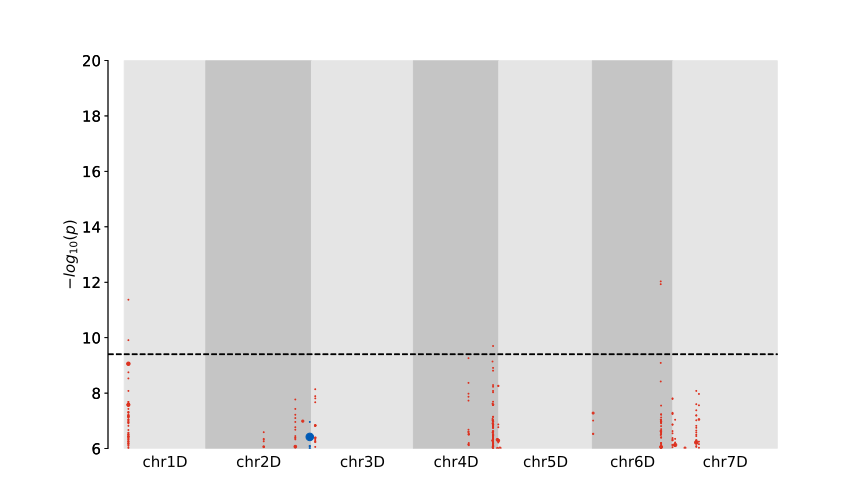
\includegraphics[scale=0.3]{images/gwas_plots/svgtopng/gh_mn_plot.png}
                \label{Fig:gh_mn_peak}
        \end{subfigure}
        \caption{Manhattan plots of the results of our GWAS analysis for leaf manganese content in \textit{Aegilops tauschii}. Red dots indicate a negative correlation, while blue dots denote a positive correlation. The top two plots show the results for the outdoor growing environments, and the bottom plot is the glasshouse environment. The dotted line represents the bonferroni-corrected significance threshold.}
        \label{Fig:mn_peak_plot_old}
\end{figure}
}

\clearpage

\chapter{Conclusion}
\section{Research Outcomes}

My aim with this thesis was to advance our understanding of how silicon-based plant traits may be applied to agriculture. To this end, I identified two separate problems that currently limit uptake and dissemination of silicon research into the broader agricultural context: 1) limited applicability of fundamental research into induced silicon uptake to crop plants, and 2) a limited understanding of the genetic basis of variation in silicon content among genotypes of a common species. Based on the exciting findings of rapid silicon accumulation in \textit{Brachypodium distachyon}, I attempted to replicate this pattern of silicon uptake in cereal crops, in the hopes that this would spur further research into silicon-based crop defences. In the growing conditions I used, I did not observe rapid silicon accumulation, but did observe variation in silicon and phenolic compound levels among the four crop species I tested. We also documented the significant variation of silicon content among common cultivars of these cereal species.

For my GWA study, we observed significant variation in silicon and manganese content between sites. Though we failed to find robust genotype-phenotype links for either silicon or manganese, we did identify one gene that is associated with variation in leaf manganese content. Additionally, by working with a previously developed diversity panel, we hope that our findings will be easily integrated into future work on this topic.

\section{Limitations and Future Directions}

A number of limitations with my study design and experimental methods should be noted. Though I was ultimately unsuccessful in my attempts to induce rapid silicification, I identified several factors that could have led to the discrepancies between previous research and my own. We utilized a single herbivore species in our treatments. Plants modulate their defensive responses based on the identity of the attacker, and it is likely that using different species or multiple species would yield different outcomes. Some of the insects in my treatments did not initiate feeding, despite our best efforts to maximise the likelihood of herbivory, and this reduced our sample size for the experiment. Finally, it is likely that the growth media we used for the study imposed some silicon limitation on our plants. This limitation may have prevented rapid uptake of silicon, as there might just not have been enough in the soil to meet the demands of the plant. Future research should explicitly investigate the silicon availability of commercially available plant growth media, as nearly all plants can respond positively to silicon. Additionally, we used a single time point to test for rapid silicon accumulation. It is possible that we pre-empted silicon uptake in our plants, and had we waited longer, we would have seen a clear signal of silicon uptake in response to our treatments. Future studies would provide immense utility to the field if they were to investigate silicon uptake at regular intervals between 6- and 48-hours post induction, as we still lack replicated data on this time interval. 

For the GWA study, we may have limited our ability to detect important marker-trait associations through the use of multiple growing environments. Though multiple growing environments are often used to prove the durability of a given marker-trait association through genotype by environment interactions, the highly exploratory nature of our work would have benefited from a deeper and narrower experimental design, where we had more replicates in a single environment. We are left with few markers to investigate, but future work could take the genotypes we identified as having high and low silicon and develop a mapping population using experimental crosses. The increased level of control this design would bring might allow for the discovery of markers associated with silicon content. Similar studies in wheat and rice have yielded promising results, and there is no reason to believe that \textit{Aegilops tauschii} would not have similar genes that influence silicon uptake.

For both experiments, adding soil chemistry data would help to improve our understanding of our observations. In both chapters, we posit that the potting mix may have low-levels of plant-available silicon. Without testing this directly, this remains speculative, and prevents concrete conclusions about our results. In the GWA study, having soil chemistry data to compare and contrast the three growing sites would help to clarify to what extent differences in phenotype are driven by the environment, genotypic effects, or an interaction of the two. An additional limitation of the GWA experiment is our lack of XRF calibrations for manganese and other metals. Adding these data would allow further regressions of silicon and other root carboxylate mobilized metals, which may help strengthen our link between silicon uptake and manganese content in the plants.

\printbibliography

\end{document}